\documentclass[11pt]{article}
\usepackage[margin=1in]{geometry}
\usepackage{amsmath,amssymb,amsthm}
\usepackage{hyperref}
\usepackage{graphicx}

\newtheorem{theorem}{Theorem}
\newtheorem{lemma}{Lemma}
\newtheorem{remark}{Remark}

\newcommand{\R}{\mathbb{R}}
\newcommand{\E}{\mathbb{E}}
\newcommand{\Lip}{\mathrm{Lip}}
\newcommand{\Proj}{\mathsf{Proj}}
\newcommand{\vol}{\mathrm{vol}}

\title{A dimension-free partial answer to the affine projection question on \texorpdfstring{$\ell_p^n$}{ell_p^n} balls}
\author{Run \texttt{fa\_banach\_001}, lane 8}
\date{2026-06-23}

\begin{document}
\maketitle

\section*{Source and target question}

The source is Tuomas Hytonen and Assaf Naor, \emph{Heat flow and quantitative differentiation}, arXiv:1608.01915.  In Section 1.F.1, Question 19 asks whether the affine orthogonal projection on an isotropic convex body is bounded on Lipschitz maps.  In the source notation, if $(X,\|\cdot\|_X)$ is $n$-dimensional, $B_X$ is in isotropic position with isotropic constant $L_X$, and $\Proj$ is the $L_2(B_X)$-orthogonal projection onto affine functions,
\[
\Proj f(x)=\int_{B_X} f(z)\,dz+\frac{1}{L_X^2}\sum_{j=1}^n x_j\int_{B_X} z_j f(z)\,dz,
\]
the question is whether, for every Banach space $Y$ and every Lipschitz $f:B_X\to Y$,
\[
\|\Proj f\|_{\Lip(B_X,Y)}\lesssim \|f\|_{\Lip(B_X,Y)}
\]
with a universal implicit constant.  The source also records that the problem is equivalent to a scalar Wasserstein symmetry estimate.

\begin{center}
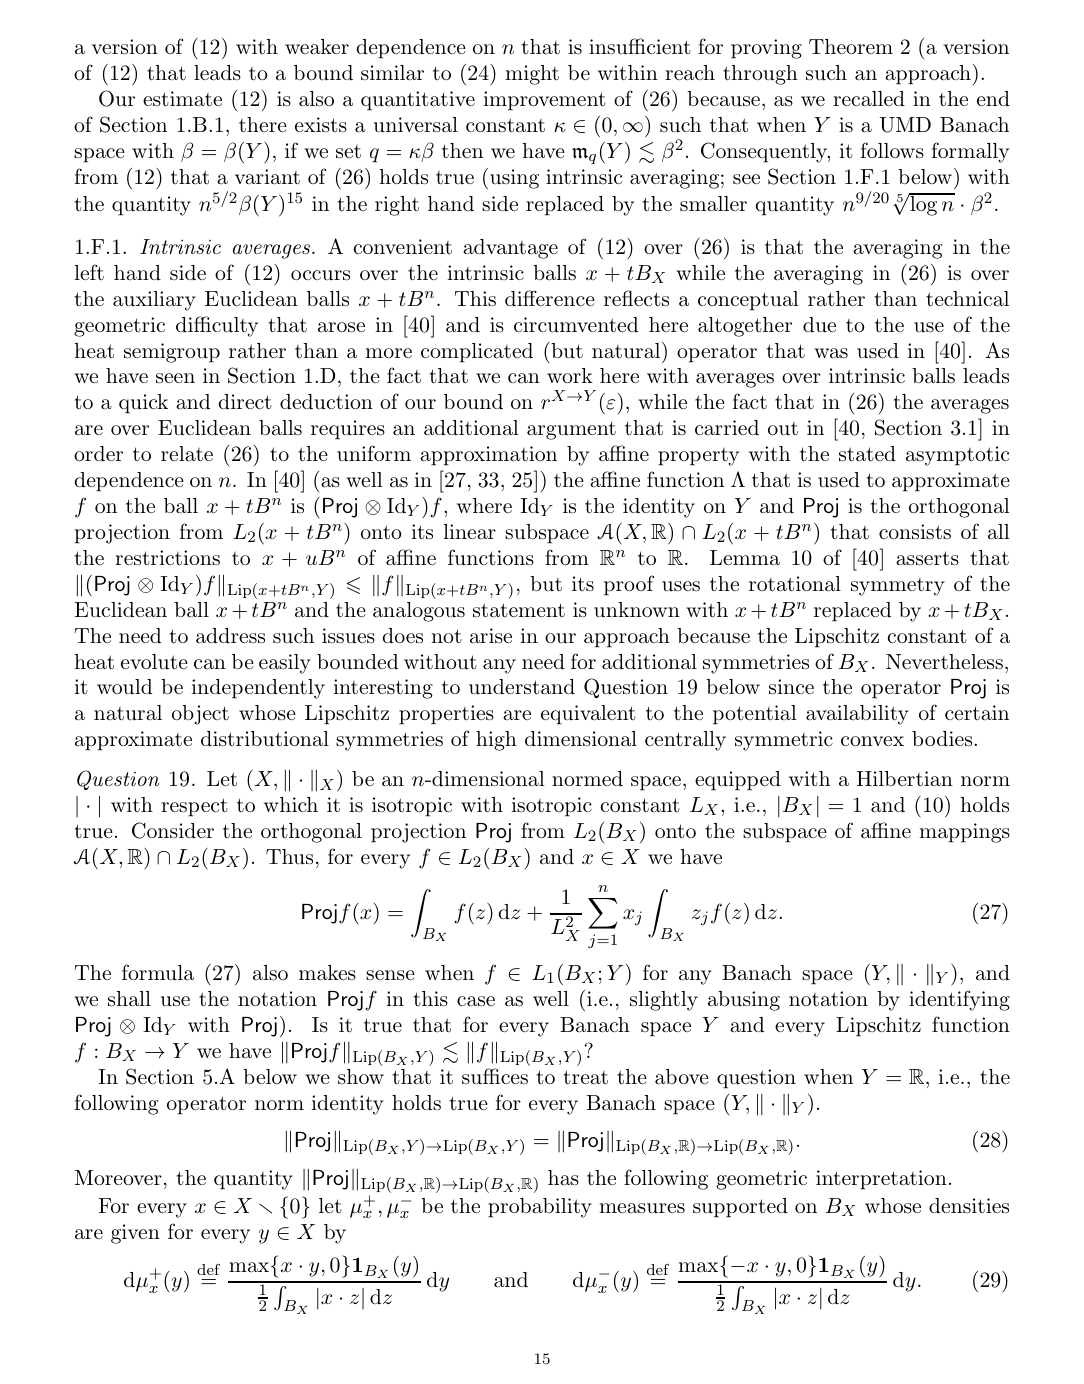
\includegraphics[width=0.92\linewidth]{figures/open_problem_page15.png}
\end{center}

\section*{Result}

This packet proves a dimension-free affirmative answer for the classical finite-dimensional $\ell_p$ balls.

\begin{theorem}
\label{thm:lp-proj}
Fix $p\in[1,\infty]$.  For every $n\in\mathbb N$, let $X=\ell_p^n$, and put its unit ball in the volume-normalized isotropic position used in Question 19 of Hytonen--Naor.  Let $Y$ be any Banach space.  Then the affine projection $\Proj$ satisfies
\[
\|\Proj f\|_{\Lip(B_{\ell_p^n},Y)}
   \le C_p \|f\|_{\Lip(B_{\ell_p^n},Y)}
\]
for every Lipschitz map $f:B_{\ell_p^n}\to Y$, where $C_p$ is independent of $n$.  For $p=\infty$ one may take $C_\infty=3/2$.  For each finite $p$, one may take
\[
C_p=\sup_{n\ge 1}
\frac{1}{2\sigma_{p,n}^2}
\left(
\frac{\Gamma(3+1/p)\Gamma(1+n/p)}
{\Gamma(1+1/p)\Gamma(3+n/p)}
\right)^{1/p},
\]
where
\[
\sigma_{p,n}^2=
\frac{\Gamma(3/p)\Gamma(1+n/p)}
{\Gamma(1/p)\Gamma(1+(n+2)/p)}.
\]
The displayed supremum is finite for every fixed $p<\infty$.
\end{theorem}

\section*{Proof intuition}

For a centrally symmetric body the affine projection is controlled, in the scalar case, by covariances of the form $\int z_j f(z)\,dz$.  On an $\ell_p$ ball, each such covariance has a one-dimensional integration-by-parts representation along the $j$th coordinate:
\[
\int z_j f(z)\,dz=\int W_j(z)\,\partial_j f(z)\,dz,
\]
where $W_j$ is the gap between the square of the coordinate slice radius and $z_j^2$.  If scalar $f$ is $1$-Lipschitz for the $\ell_p$ metric, then $|\nabla f|_{\ell_{p'}}\le 1$ a.e.  Thus a linear combination of the covariance terms is bounded by an $L_p$ moment of the weights $W_j$.  That moment is of the same order as the coordinate variance of the uniform measure on the $\ell_p$ ball, uniformly in the dimension.  Dividing by the covariance normalization in the projection formula gives the dimension-free scalar bound; the Hytonen--Naor scalar-to-Banach identity then gives the stated result for every target $Y$.

\section*{Proof}

By equation (28) in the source paper, the Lipschitz operator norm of $\Proj$ with arbitrary Banach target $Y$ is equal to its scalar-valued Lipschitz operator norm.  It is therefore enough to prove the theorem for scalar-valued Lipschitz functions.  We work with the standard unit ball
\[
K_p^n=\{z\in\R^n:\|z\|_p\le 1\}
\]
and normalized Lebesgue probability measure on it.  A common dilation of the body changes the covariance and the Minkowski functional in opposite ways and leaves the Lipschitz operator norm of $\Proj$ unchanged.  The standard Euclidean structure is isotropic for $K_p^n$ by sign and permutation symmetry, after volume normalization.

Let $Z$ be uniformly distributed on $K_p^n$.  For $p<\infty$, write
\[
\sigma_{p,n}^2=\E Z_1^2.
\]
For smooth scalar $f:K_p^n\to \R$, the affine projection has linear part
\[
h\mapsto \frac{1}{\sigma_{p,n}^2}\E[(h\cdot Z)f(Z)].
\]
Smoothness is harmless: the general scalar Lipschitz case follows by the usual mollification argument on slightly smaller balls and passage to the limit, or equivalently by applying the following integration-by-parts identities to a.e. classical derivatives.

Fix $j$ and freeze all coordinates except $z_j$.  If
\[
A_j(z)=\left(1-\sum_{i\ne j}|z_i|^p\right)^{1/p},
\]
then along that slice $z_j\in[-A_j,A_j]$.  Integration by parts gives
\[
\int_{-A_j}^{A_j} t\, f(\ldots,t,\ldots)\,dt
=\frac12\int_{-A_j}^{A_j}(A_j^2-t^2)\,\partial_j f(\ldots,t,\ldots)\,dt.
\]
Consequently
\[
\E[Z_j f(Z)]=\E[W_j(Z)\partial_j f(Z)],
\qquad
W_j(Z)=\frac{A_j(Z)^2-Z_j^2}{2}.
\]

Let $h\in\ell_p^n$.  Since $|\nabla f(Z)|_{\ell_{p'}^n}\le \|f\|_{\Lip}$ almost everywhere,
\[
\begin{aligned}
\left|\E[(h\cdot Z)f(Z)]\right|
&=\left|\E\sum_{j=1}^n h_j W_j(Z)\partial_j f(Z)\right|\\
&\le \|f\|_{\Lip}\,
\E\left(\sum_{j=1}^n |h_j|^p W_j(Z)^p\right)^{1/p}\\
&\le \|f\|_{\Lip}\,\|h\|_p\,(\E W_1^p)^{1/p}.
\end{aligned}
\]
Here the last step uses Jensen's inequality and symmetry of the $W_j$.
Thus
\[
\|\Proj f\|_{\Lip(K_p^n,Y)}
\le
\frac{(\E W_1^p)^{1/p}}{\sigma_{p,n}^2}\|f\|_{\Lip(K_p^n,Y)}.
\]
For $p=1$ this already yields the sharper bound $1$, because $\E W_1=\E Z_1^2$.

For $1<p<\infty$, use $0\le W_1\le A_1^2/2$.  A beta-integral calculation gives
\[
\E A_1^{2p}
=
\frac{\Gamma(3+1/p)\Gamma(1+n/p)}
{\Gamma(1+1/p)\Gamma(3+n/p)}
\]
and
\[
\sigma_{p,n}^2=\E Z_1^2
=
\frac{\Gamma(3/p)\Gamma(1+n/p)}
{\Gamma(1/p)\Gamma(1+(n+2)/p)}.
\]
Therefore
\[
\frac{(\E W_1^p)^{1/p}}{\sigma_{p,n}^2}
\le
\frac{1}{2\sigma_{p,n}^2}
\left(
\frac{\Gamma(3+1/p)\Gamma(1+n/p)}
{\Gamma(1+1/p)\Gamma(3+n/p)}
\right)^{1/p}.
\]
The standard gamma-ratio estimate $\Gamma(t+a)/\Gamma(t+b)\asymp_{a,b}t^{a-b}$ shows that this expression is bounded in $n$ for each fixed $p<\infty$.

It remains to record the endpoint $p=\infty$.  Now $K_\infty^n=[-1,1]^n$ and $\sigma_{\infty,n}^2=\E Z_1^2=1/3$.  One-dimensional integration by parts gives
\[
\E[Z_j f(Z)]
=\E\left[\frac{1-Z_j^2}{2}\partial_j f(Z)\right].
\]
For $h\in\ell_\infty^n$,
\[
\left|\E[(h\cdot Z)f(Z)]\right|
\le
\|f\|_{\Lip}\,
\E\left\|\left(h_j\frac{1-Z_j^2}{2}\right)_{j=1}^n\right\|_\infty
\le \frac12\|h\|_\infty\|f\|_{\Lip}.
\]
After division by $\sigma_{\infty,n}^2=1/3$, this gives
\[
\|\Proj f\|_{\Lip(K_\infty^n,Y)}\le \frac32\|f\|_{\Lip(K_\infty^n,Y)}.
\]
This proves the theorem.

\section*{Verification and limitations}

The proof is exact for the whole $\ell_p^n$ scale and all Banach targets $Y$.  It does not answer Question 19 for arbitrary isotropic convex bodies.  The constants for finite $p$ are not optimized; for instance, the Euclidean ball has a better bound by rotational symmetry.

The script \texttt{code/check\_gamma\_constants.py} numerically samples the explicit finite-$p$ Gamma-ratio bound for representative $p$ and $n$.  This is only a sanity check; the dimension-free assertion follows from the displayed Gamma-ratio asymptotics.

Novelty check: the cheap run indexes had no hit for arXiv:1608.01915, the paper title, or distinctive `Q:proj lip' phrases.  A bounded web search for exact affine-projection and Wasserstein-symmetry phrases found the source arXiv page but no later direct answer.  This is therefore recorded as a likely-new partial result, subject to human review.

\section*{References}

\begin{itemize}
\item T. Hytonen and A. Naor, \emph{Heat flow and quantitative differentiation}, arXiv:1608.01915, 2016.
\end{itemize}

\end{document}
